% !TeX root = main.tex


\chapter{State of the art and a theoretical Background}
\label{chap:2}
Chapter \ref{chap:2} introduces the theoretic baselines for data acquisition, data metrics as well as standardized data formats in which to save metadata.


Topics to consider when starting the Sensor Health Monitoring process are mainly that of providing a structured overview of the Sensor Metadata which in itself consists of many layers as a dynamically generated set of metadata is desired. This should be able to accomodate changing Data Acquisitioning (DAQ) System configuration changes.
Consideration is given to the SOIL data model and its' ability to accomodate the many demands that are expected of sensor data management. \cite{behrens_domain-specific_2021}
The second major part to consider is that of physical crossrelations and \"deep checks\" which are a experimental mode of checking for inconsistencies among the data.
Major research and implementation work shall go into developing a dynamic model that is generated from the data and then checks back upon the data for possible discrepancies. This approach is chosen as it is estimated to be the most structured approach for a first prototype.


This topic shall give an overview over the state of the art technology as well as systems and describe the systems employed by this work. Structuring the data


\begin{figure}[h]
    \centering
    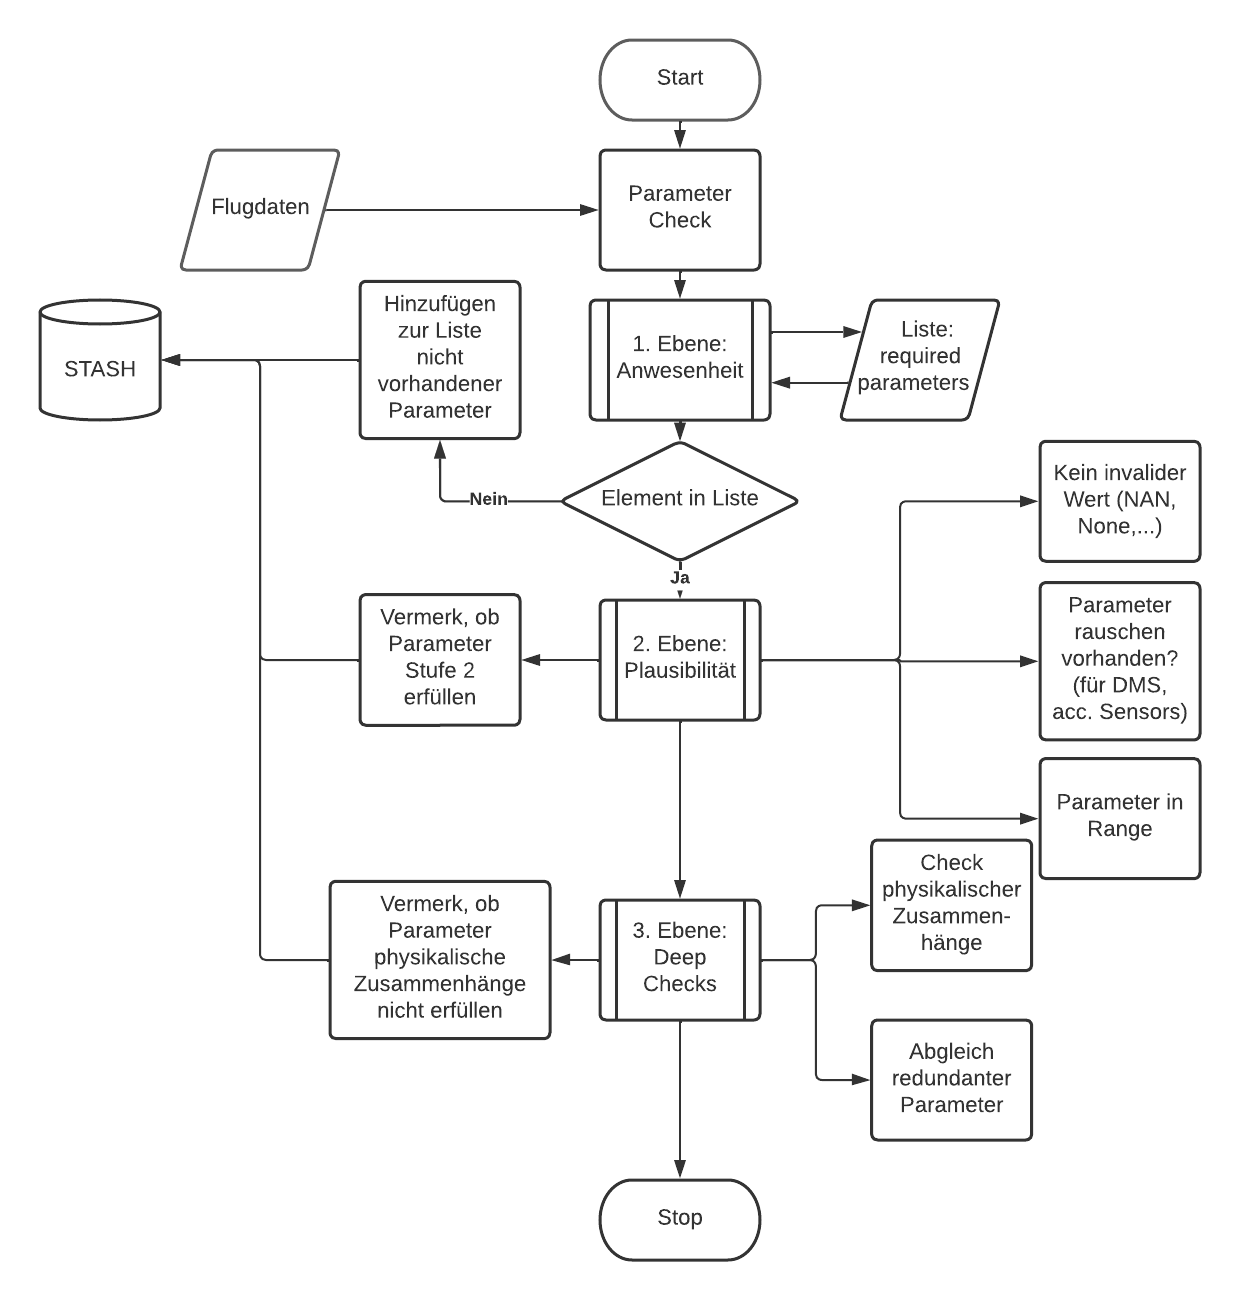
\includegraphics[width=1\textwidth]{SensorHealthMonitoring}
    \caption{}
    \label{fig:shm}
\end{figure}


\section{What is SHM?}

-detect failures
-

When talking about Sensor Health Monitoring (SHM) generally one requirement is made which is to detect failures and suspicious behaviours within a system. The failures then need to be quantified to allow writing algorithms to detect them. If one had a sensor value that differed strongly from its expected values a decision needed to be made how much the sensor value differed from the expected value and where the system would receive the information from. This and further considerations are examined in the following chapter to generate a broad overview over the topic of Sensor Health Monitoring and Fault Detection.

\subsection{Scope}
In addition to detecting faults it is also necessary for a SHM to display faults to the systems operator. This may happen in the shape of a display interface or a dashboard that generates fault and reliability ratings. Condensing information for operators is also a necessary part of SHM since suspicious occurences may be frequent and raw information about events is less helpful than already preprocessed data.


%%%scope of this work
Within this chapter various algorithms and methods that may be used to detect faults are presented first and then followed by considerations in the direction of metadata. Standards for metadata as well as new propositions are examined and the skystash architecture which is used for data hosting as well as analytic tasks is presented.


\subsection{Requirements}
□ Notwendig
-detect errors within previous flights.
-develop a toolchain that accesses configuration data for parameters
-find a format to communicate metadata as well as SHM findings
-develop first on a small batch size
□ optional
-develop smarter algorithms
-include all parameters

\section{Fundamentals}

%\subsection{Isermann}
Lets talk about Semantics and descriptors of data/metadata. Hence, a quick insert about semantics

\subsection{Semantics}
Semantics are defined in various way by various people. One definition that has found some acceptance is the definition by Metzlers Lexikon which relies on theories by Blackburn and Kutschera. \cite{shoemaker_spreading_1987,kutschera_sprachphilosophie_1975}


First off, semiotics from the greek σημεῖον, semeion for sign, describes the theory of signs and their usage. Semiotics is divided into the areas semantics, syntactics and pragmatics. Within the definition at hand syntactics is given as the internal structure of signs within sign systems, pragmatics are defined as the theory of sign usage effectively thinking about how interaction with signs works.
Finally, semantics define the relationship between signs and described objects. They work by allocating a structure/model to a predefined expressions

\begin{figure}
    \centering
    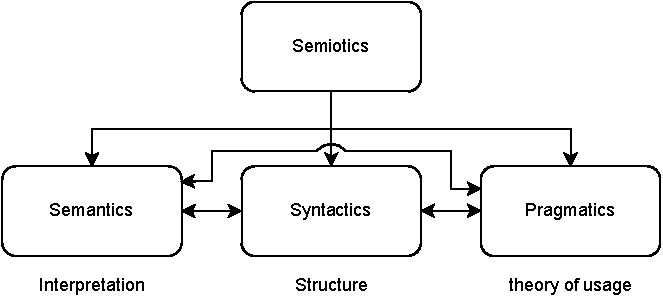
\includegraphics[width=.7\textwidth]{03_figures/semiotics.pdf}
    \caption{Semiology, according to \textcite{kutschera_sprachphilosophie_1975} and \textcite{shoemaker_spreading_1987}}
\end{figure}


And now to the actual semantics that have been mentioned previously:

\subsection{Metadata descriptors}


\begin{figure}[ht]
    \centering
    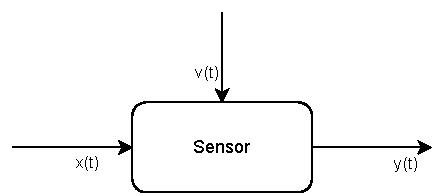
\includegraphics[width=1\textwidth]{basic_error_abb}
    \caption{Sensor Signal with control systems}
    \label{fig:basic_error_abb}
\end{figure}
\begin{figure}[ht]
    \centering
    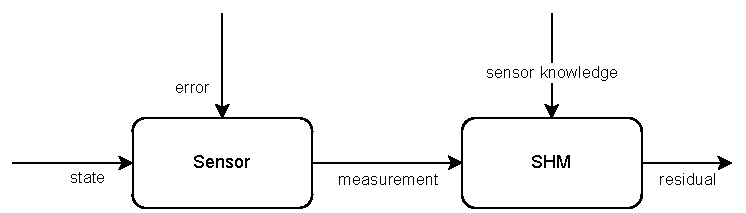
\includegraphics[width=1\textwidth]{basic_error_filter}
    \caption{Sensor Signal Filter}
    \label{fig:basic_error_filter}
\end{figure}


Unambiguous terms are needed to provide clear information within the sensor health monitoring data structure. This is needed in regards to basic terms like semantics as well as data metrics. In the following, industry standards and definitions are collected to accompany this work.






1What are metadata descriptors

u-is the input
x-is the system state
y-is the sensor value
n-noise


2what are metadata descriptors


No clear, fully unambiguous and precise definition exists for most of following terms. However some assumptions have been made by e.g. isermann et al[ise97] within trends and apps.. in discussion with vdi/vde committees and the reliability, availability and maintainability (RAM) dictionary. Definitions are classified as:

deviation: difference to a reference value


\begin{itemize}
    \bfseries
    \item states and signals (chapter \ref{chap:metadata_states})
    \item functions (chapter \ref{chap:metadata_functions})
    \item models (chapter \ref{chap:metadata_models})
    \item system properties (chapter \ref{chap:metadata_system_properties})
\end{itemize}

\subsection{States and Signals}
Basic descriptors for occurences in signals (states). Faults are definedWithin this definition it is however not clearly defined

\label{chap:metadata_states}
\begin{table}[!h]
    \centering
    \begin{tabular}{@{}ll@{}}
        \toprule
        descriptor   & description                                                                           \\ \midrule
        fault        & unpermitted deviation of one subset of the system                                     \\
        failure      & permanent interruption                                                                \\
        malfunction  & intermittent regularity                                                               \\
        disturbance  & unknown, uncontrolled input                                                           \\
        perturbation & input, leading to temporary departure from steady state                               \\
        error        & deviation between measurement and true, specified, theoretically correct value        \\     & $y_e = \bar{y} -y$ \\
        residual     & fault indicator based on deviations between measurements and model-based calculations \\     & $\hat{y} = \bar{y} -y_m$ \\ \bottomrule
    \end{tabular}
    \caption{states and signals}
    \label{tab:states_and_signals}
\end{table}

\subsection{functions}
\label{chap:metadata_functions}
\begin{table}[!h]
    \centering
    \begin{tabular}{@{}ll@{}}
        \toprule
        descriptor           & description                                                                                                     \\ \midrule
        fault detection      & determination fault presence                                                                                    \\
        fault isolation      & Determination fault properties: kind, location, time of detection                                               \\
        fault identification & determination of size and time-variant behaviour of fault                                                       \\
        fault diagnosis      & includes fault detection, isolation, identification                                                             \\
        monitoring           & real-time determination of possible physical conditions and recognition and indication of behavioural anomalies \\
        Supervision          & monitoring and taking actions to maintain operation during faults                                               \\
        protection           & means by which potentially dangerous behaviours are suppressed if possible or how consequences are avoided      \\ \bottomrule
    \end{tabular}
    \caption{functions}
\end{table}

\subsection{models}
\label{chap:metadata_models}

\begin{table}[!h]
    \centering
    \begin{tabular}{@{}ll@{}}
        \toprule
        descriptor            & description                                                                     \\ \midrule
        quantitative          & describe system in quantitative mathematical terms                              \\
        qualitative           & describe system in causalities and if-then rules                                \\
        diagnostic            & link specific inputs (symptoms) to outputs (faults)                             \\
        analytical redundancy & determine a quantity in an additional way by using a mathematical process model \\ \bottomrule
    \end{tabular}
    \caption{models}
\end{table}

\subsection{system properties}
\label{chap:metadata_system_properties}


\begin{table}[!h]
    \centering
    \begin{tabular}{@{}ll@{}}
        \toprule
        descriptor     & description          \\ \midrule
        MTTF=1/\lambda & Mean time to failure \\
        \lambda        & rate of failure      \\
        MTTR = 1/\mu   & mean time to repair  \\
        \mu            & rate of repair       \\ \bottomrule
    \end{tabular}
    \caption{system properties}
\end{table}



\begin{table}[!h]
    \centering
    \begin{tabular}{@{}ll@{}}
        \toprule
        descriptor   & description                                                                               \\ \midrule
        reliability  & ability to perform a function, measure $MTTF$, with $\lambda$ as rate of failure per hour \\
        safety       & ability of a system not to cause danger to persons, equipment and environment             \\
        availability & $A=\frac{MTTF}{MTTF + MTTR}$                                                              \\ \bottomrule
    \end{tabular}
    \caption{system properties}
\end{table}


data quality:
reliability (isermann)
availability (isermann)
accuracy


3what are metadata descriptors

they need to be clearly defined as they have been now to set a common ground upon which this work can be built.

%\subsection{Integrity, Reliability and Validity based on GNSS or NORMS von Lars}
Data according to ISO 8000 cite [ISO22]
iso5725:
-accuracy(validity)+precision(reliability)
Also see precision and accuracy definition \cite[S.33ff.]{smith_scientist_nodate}



Other measures for various positioning systems are found in \textcite{faa_federal_radionavigation_plan_2008}. Also, similar definitions are found as defined in \textcite{isermann_fault-diagnosis_2011}
$Reliability = 1-Probability_{Failure}$
\cite[B.1.5]{faa_federal_radionavigation_plan_2008}

B.1.10: Integrity: Display when system should not be used due to potential errors.

Validation: Black Box Testing. Results match expectations
Verification: White Box Testing. Establish algorithm's truth

\subsection{Statistics}
\cite{smith_scientist_nodate}
\begin{figure}[h]
    \centering
    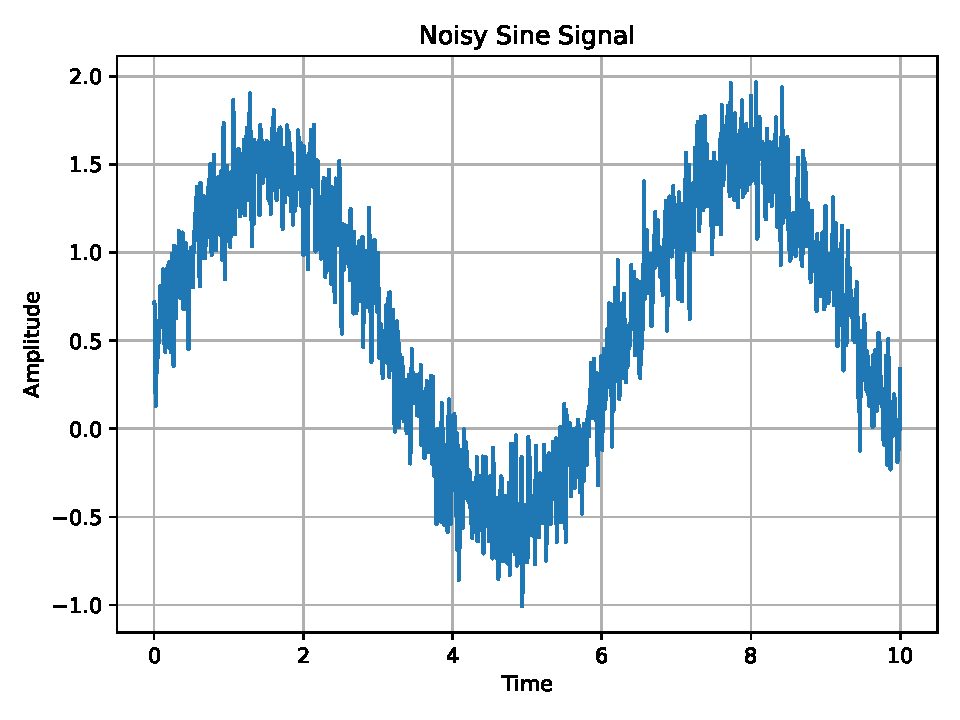
\includegraphics[width=.7\textwidth]{python_functions/images/statistic_functions_clean}
    \caption{Noisy Sine Signal}
    \label{fig:statistics_clean}
\end{figure}
\begin{figure}[h]
    \centering
    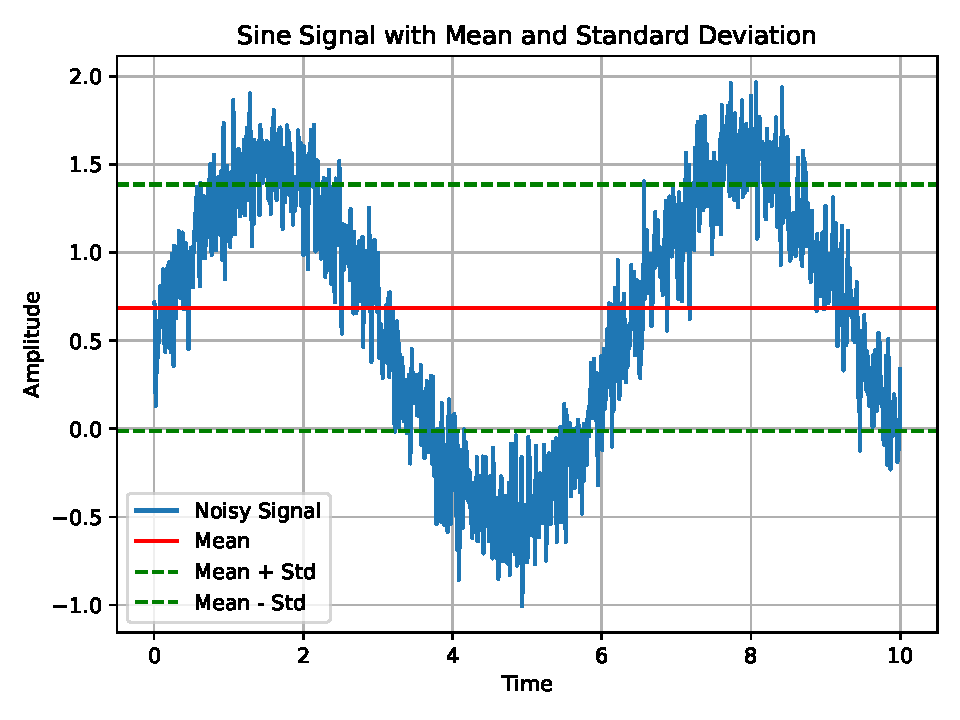
\includegraphics[width=.7\textwidth]{python_functions/images/statistic_functions_basic}
    \caption{Sine Signal with mean and standard deviation}
    \label{fig:statistics_basic}
\end{figure}
\begin{figure}[h]
    \centering
    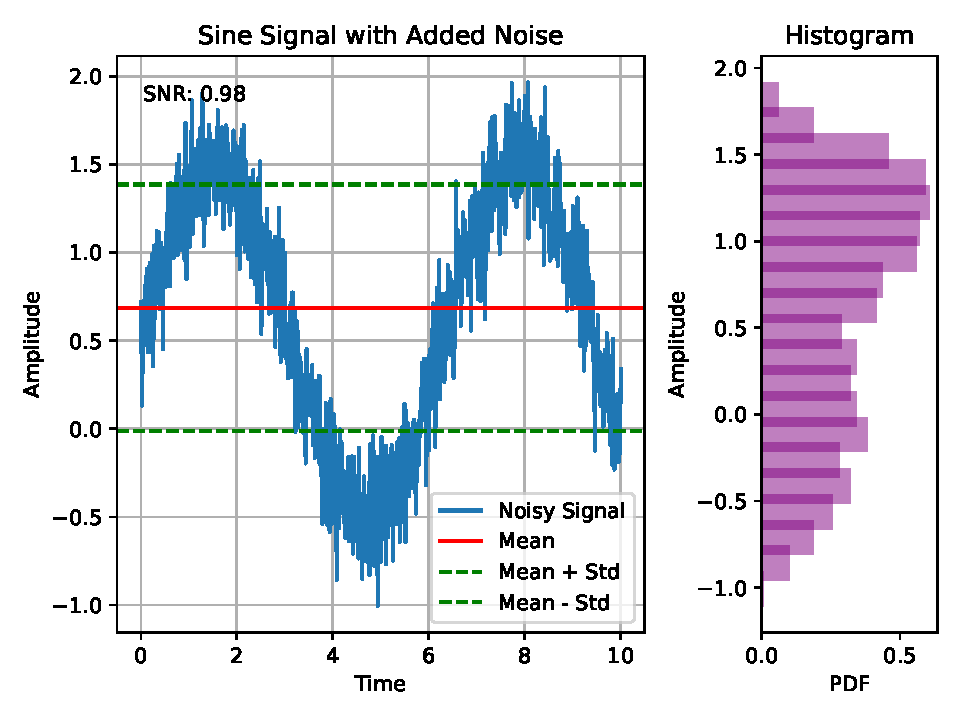
\includegraphics[width=.7\textwidth]{python_functions/images/statistic_functions_full}
    \caption{Sine Signal full analysis with mean, stdev, SNR and Histogram}
    \label{fig:statistics_full}
\end{figure}


Definition Fault Detection + Fault Diagnosis (Fault-Diagnosis Applications)


Signal properties are examined for a given signal in figure \ref{fig:statistics_clean}





Sensors generally produce errors within expected forms of output.
-Noise
-Measure using Covariance --> autocovariance
-Offset
-No response

Statistical representation of:
Mean

\cite[S.13-17]{smith_scientist_nodate}

Time continuous mean
\begin{equation}
    \label{eq:mean_cont}
    \mu=\frac{1}{T} \cdot \int_T x(t) d t
\end{equation}
Time discrete mean:
\begin{equation}
    \label{eq:mean_disc}
    \mu=\frac{1}{N} \cdot \sum_{i=1}^{N} x_i
\end{equation}




The variance $\sigma^2$ is a metric for the signal's behaviour. It expresses the mean squared deviation from the mean.

Time
\begin{equation}
    \label{eq:var_cont}
    \sigma^2=\frac{1}{T} \cdot \int_T[x(t)-\mu]^2 d t\\
\end{equation}

\begin{equation}
    \label{eq:var_disc}
    \sigma^2=\frac{1}{N} \cdot \sum_{i=0}^{N}\left[x_i-\mu\right]^2
\end{equation}

The standard deviation is derived from the variance. Its value gets square-rooted to better represent the power (magnitude of the amplitude).

Standard Deviation
\begin{equation}
    \label{eq:stdev_disc}
    \sigma = \sqrt{\sigma^2}
\end{equation}

Mean and the standard deviation don't represent the desired metrics in some use cases. Rather more important is a comparison between the two. Hence, the Signal-to-Noise ratio (SNR) is used to compare and condense the mean and standard deviation by dividing the mean by the standard deviation.

\begin{equation}
    \label{eq:snr}
    SNR=\frac{\mu}{\sigma}
\end{equation}
Another parameter is the coefficient of variation (CV) which is the standard deviation divided by the mean and multiplied by 100\%.

\begin{equation}
    \label{eq:coeff_var}
    CV = \frac{\sigma}{\mu}100\%
\end{equation}

An arising problem based on the SNR and CV are however that they scale based on the mean value. Should the mean value lie at about 0 for e.g. a sensor of an aircraft control surface, the signal to noise ratio will be relatively high compared to an acceleration sensor in z axis with a constant offset of 1g

Practical example for mean and standard deviation in a given signal are overlayed in figure \ref{fig:statistics_basic}


To evaluate a signal according to the quantities the next logical step for statistic Histogram

probability mass function

\begin{equation}
    f(x)=\frac{1}{\sqrt{2 \pi \sigma^2}} e^{-\frac{(x-\mu)^2}{2 \sigma^2}}
\end{equation}


Covariance
Zeitkontinuierliche Autokovarianzfunktion
$$
\gamma(\tau)=\frac{1}{T} \cdot \int_T[x(t)-\mu] \cdot[x(t-\tau)-\mu] d t
$$
Zeitdiskrete Autokovarianzfunktion
$$
\gamma(k)=\frac{1}{N} \cdot \sum_N\left[x_i-\mu\right] \cdot\left[x_{i-k}-\mu\right]
$$

-->Autocovariance
autocov(x,x) = cov(x,x)


Correlation (Pearson coefficient)

$$\rho_{x,y} = corr(x,y)=\frac{cov(x,y)}{\sigma_x \sigma_y}$$

The maximum of a total correlation is 1 or that of a total negative correlation -1.

Total independence for $\rho_{x,y}=0$ not given since Pearson coefficient only detects linear correlations

Other correlation methods as rank-correlation (Spearman, Kendall) that detect change correlations are possible but are more complex in the implementation.


\section{Signal Discretization}

State values of the real system are never measured without some error. Upon measurement, sensor values are discretized by converting it to a digital signal. This happens in two steps that are presented in an exemplary setup in figure \ref{fig:signal_processing_setup}. In the first step the real state value gets converted into a sensor signal by measuring it within a pitot tube. Within this step, some white noise generally occurs. Within the second step the sensor value gets converted to a digital signal by feeding it into an Analog Digital Converter (ADC). During the ADC step a discretization error occurs. Based upon sampling rate discretization errors occur in time and value direction. After the transformation by both steps, the data series contain a white noise sensor error as well as a discretization error (see figure \ref{fig:signal_processing_plots}, Point 3). Great effort is made to avoid such errors. For sensor errors i.e. a nose boom is fitted to the aircraft to measure undisturbed stream conditions. For value and time discretization the resolution of the ADC is chosen to guarantee necessary parameter precision. An exemplary signal transforming process is shown in figure \ref{fig:signal_processing_plots}.

\begin{figure}[!h]
    \centering
    \begin{subfigure}{\textwidth}
        \centering
        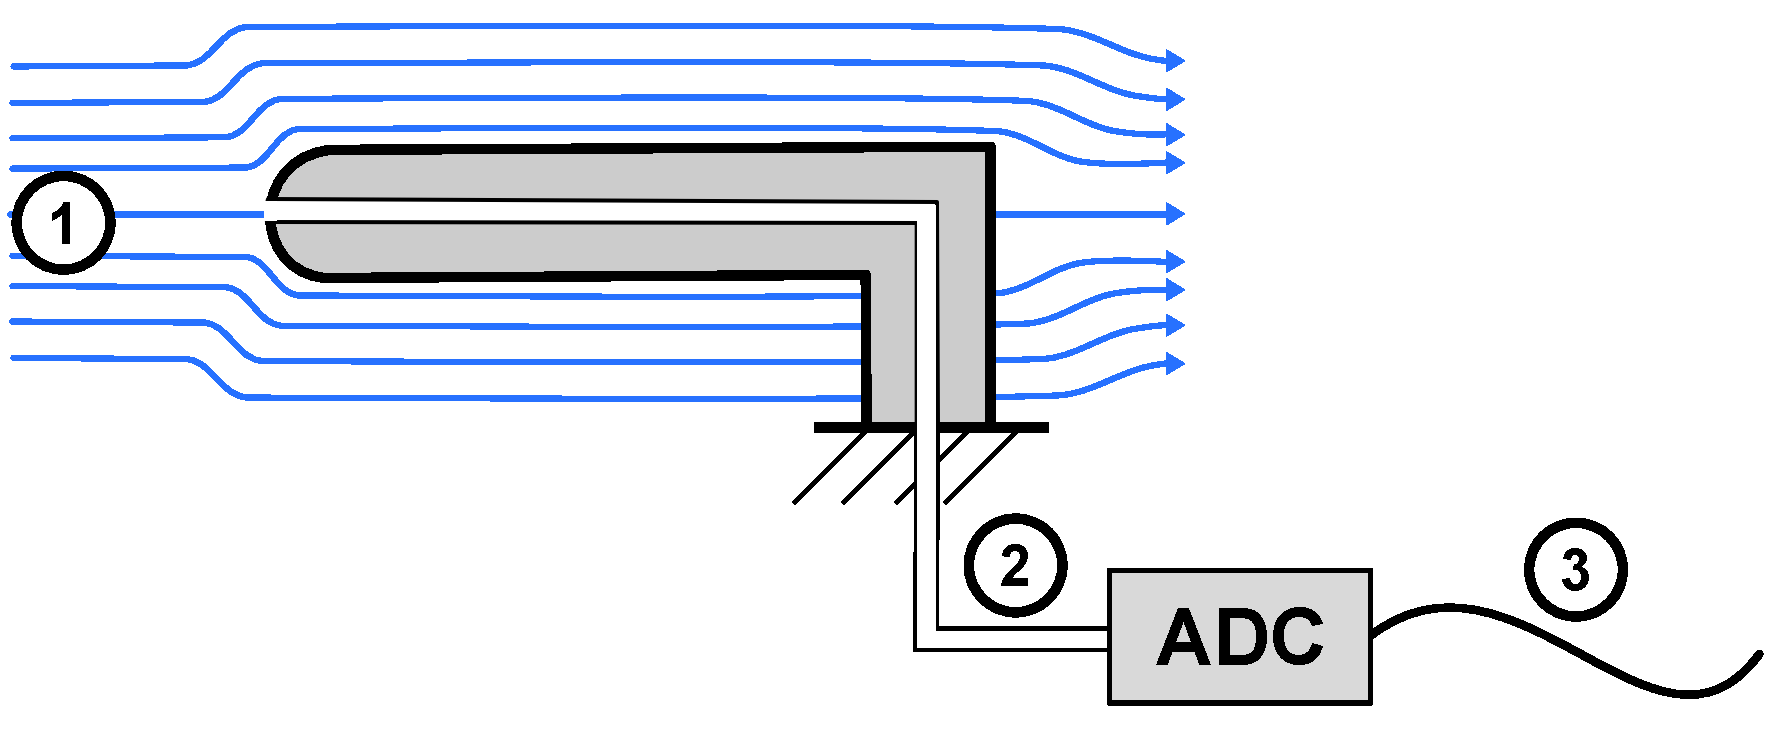
\includegraphics[width=0.8\textwidth]{03_figures/signal_recording}
        \caption{pitot tube setup for measuring dynamic pressure}
        \label{fig:signal_processing_setup}
    \end{subfigure}
    \begin{subfigure}{\textwidth}
        \centering
        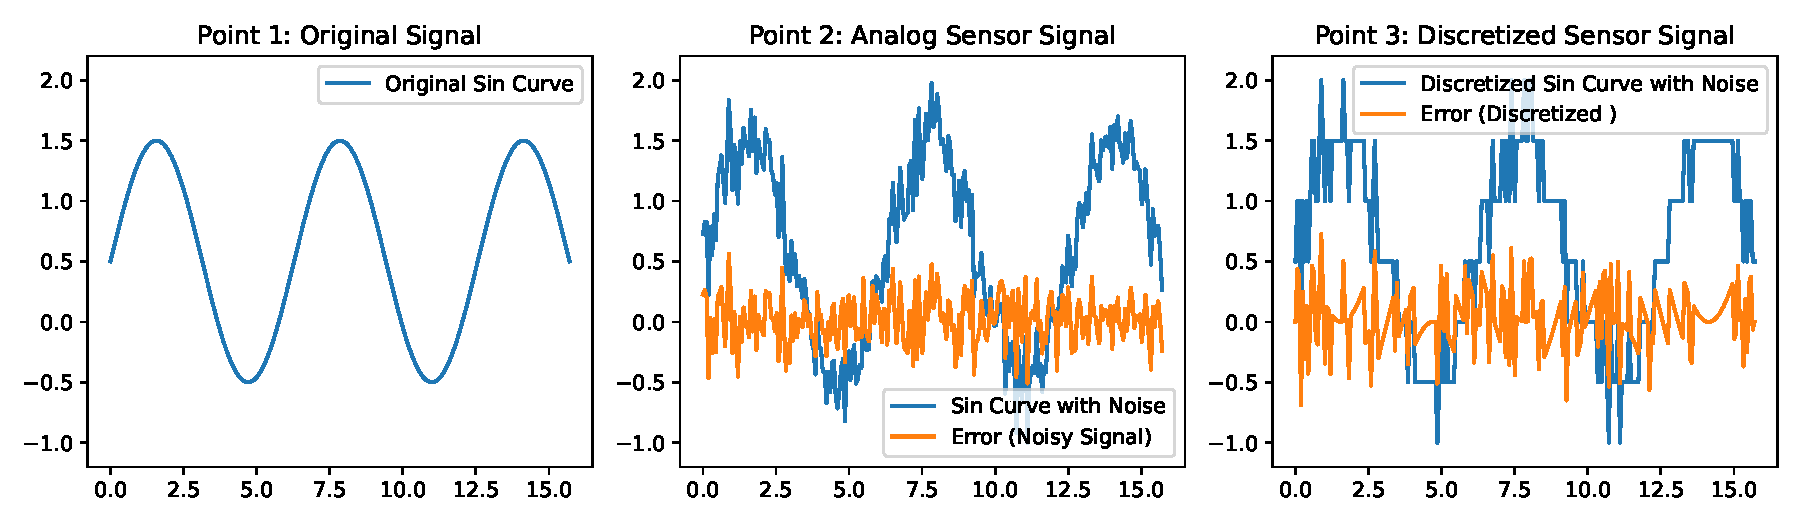
\includegraphics[width=\textwidth]{03_figures/python_functions/images/signal_processing_plots}
        \caption{Original signal into measured and discretized signal}
        \label{fig:signal_processing_plots}
    \end{subfigure}
    \caption{Simplified, exemplary signal processing flow for measurement of a dynamic pressure for real (1), analog sensor (2) and discretized sensor (3) values}
    \label{fig:signal_processing}
\end{figure}


The dynamic pressure in the air (denoted by 1) is ideally undisturbed and smooth for the actual state value. Within the sensor and stream close to the aircraft, the air is disturbed by the aircraft itself and also by the sensor, leading to the measured value at position 2. signal conversion from pressure to a voltage as well as discretization of the analog voltage to a digital signal is summarized within the ADC-Box since it is assumed that the errorwithin the pressure conversion is small compared to the errors within sensor and actual ADC. A sample signal conversion is shown within figure \ref{fig:signal_processing_plots}. Of course, errors are exaggerated for illustration since state of the art systems possess a far smaller level of sensor as well as ADC error.


All recorded sensors are present in values that are already is a process that is integral to digitally recorded sensor values.



-mention data information
-information loss through discretization

Time discretization
value quantization


\section{Previous works}

\subsection{PCA}

\subsubsection{What is PCA (Intro)}


The principal component analysis (PCA) is a method that allows to reduce the information parameters of a dataset into a few principal components. Generally this is specified as the operation of the original dataset $X_{Nxm}$ with the timesteps $N$ and the measurement parameters $m$ into the transformed principal components (PC) $T_{Nxr}$ with $r$ being amount of PCs.
This transformation is defined as:
$$T_{Nxr} = X_{Nxm}  P_{mxr}$$
with P being the permutation matrix that rotates the original data into the principal components. The overall strategy to generate a PC is shown in figure \ref{fig:pca_variance} as finding a function between two parameters $x_1$ and $x_2$ that maximizes the variance of data in the newly generated principal component. However drawbacks arise using this approach since the variance optimization only happens linearly and is not able to function for nonlinear correlations.



-originally to reduce dimensionality within a dataset \cite{handl_multivariate_2017}
-->extract maximum variance (see variance chapter) from dataset
->transform onto 2 PCs

-Application in FMEA (Isermann, fault diag) \cite{isermann_fault-diagnosis_2006}
->determine number of principal components

\subsubsection{What is PCA again? (Detail)}

%%motivation
relative minimal input. Usable results without system knowledge. Works pretty much straight out of the box

the principal component analysis is based on correlation principles and allows reduction of datasets into independent components. Applications in an aerospace context include detection of previously unknown correlations between parameters and complex interactions in aeroelastics or otherwise large datasets. It also may allow generation of rules to detect a deviation from previously correlated values. Usage however is associated with a certain effort since information needs to be preprocessed to a certain degree, reducing dimensions previous to processing in order to avoid feeding in redundant parameters. Upsides of the PCA are that it acts as a blackbox that quickly allows to reduce data onto a given set of dimensions, requiring relatively little user input.


\begin{figure}
    \centering
    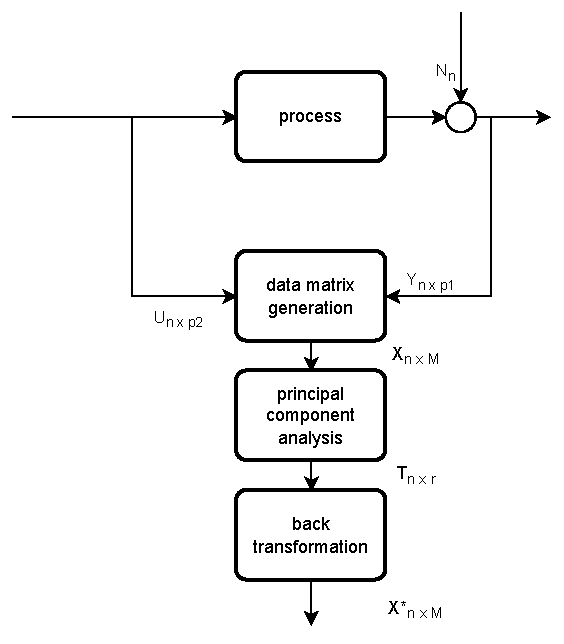
\includegraphics[width=0.8\textwidth]{pca_FD}
    \caption{Known process input U as well as Sensor Measurement Y get collected into X and fed into a PCA. N indexes timesteps.\cite[p.268]{isermann_fault-diagnosis_2006}}
    \label{fig:pca_FD}
\end{figure}


%%variance

Generally, we want to transform the Matrix X into the transformed Matrix T containing all Principal components with the count $r<m$. To perform this operation we introduce the Permutation Matrix P leading to:
$$T_{Nxr} = X_{Nxm}  P_{mxr}$$

Full derivations are available in previously cited sources (isermann, han17). Rather more important is however, that isermann presents a process for an autotuning PCA that can be used for real-time Fault Detection applications.


A principal component gets created by condensing two parameters in the direction of most variance to each other. This is a classical optimization problem


%%principal component
PCs can be created in any direction. Where input is needed however is the number of Principal components that shall be kept. A cutoff value can be defaulted to but this may not be feasible for multidimensional systems such as the flight test data that is at hand.


\begin{figure}
    \centering
    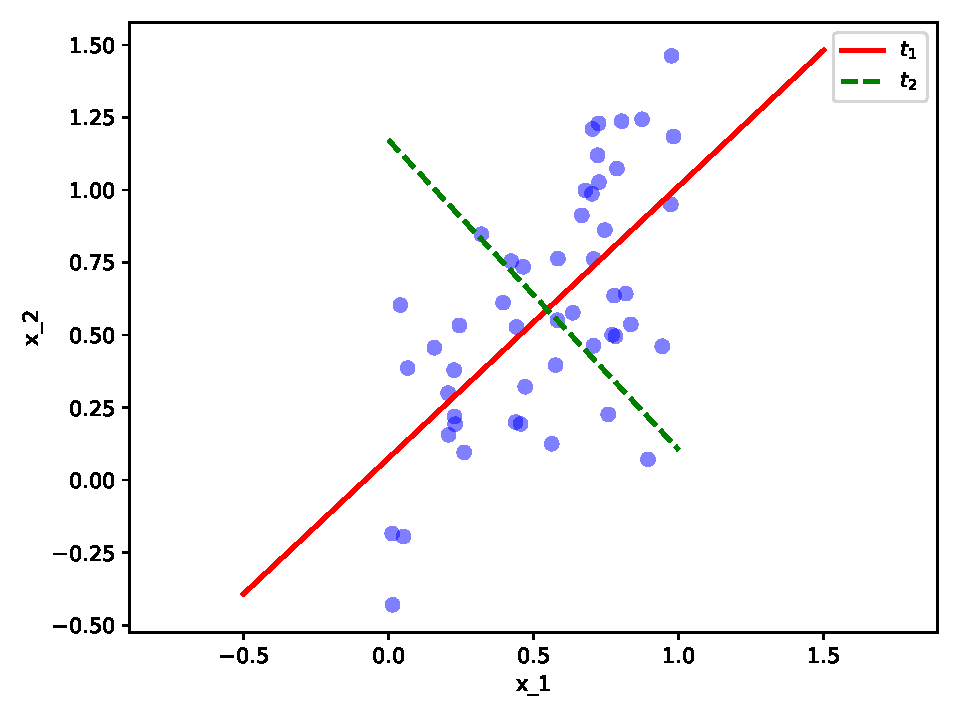
\includegraphics[width=0.8\textwidth]{python_functions/images/pca_variance}
    \caption{Parameters $x_1$ and $x_2$ get converted into principal components $t_1$ and $t_2$ by optimizing for minimal variance.}
    \label{fig:pca_variance}
\end{figure}

Eliminating a principal component becomes easy if parameters show a direct correlation such as in figure \ref{fig:pca_variance}. The gatherings of $t_2$ then mostly consist of noise and can be safely discarded.

%%pca general analysis (plots)


%%pca uses in fault detection
The PCA can be defined as a condensation of a dataset into fewer parameters. The so called principal components. These principal components can also be transformed back into the original parameters. This process can also be used to create a data model and then calculate the residual to possibly quantify the error.


2. create principal components by maximizing variance

3. for all

analogy to covariance matrix

SVD.

\subsubsection{What is PCA (Concluding remarks. Lessons learned)}

\subsection{ PTF}

\subsubsection{control systems approach}

what are state values?


Following the recipe for a modeled aircraft based on sensor data we try to simulate the parameters x and u of the aircraft with the sensor data y. Khaled shows that this approach works for linking omega_x omega_y, delta_delta(drift angle) with omega_z. and Transmissibility function  $\mathcal{T}$


The examined approaches include:
\begin{enumerate}
    \item Transmissibility functions $\mathcal{T}$ that model the system output without having to take the unknown
    system input into consideration
    \item Bond Graphs to model a physical rigid aircraft system
    \item Physical relations
    \item redundancies between sensors
\end{enumerate}

model based fault detection(isermann)
-parameter estimation (process modeling with linear or nonlinear functions, unknown process parameters are modeled by residual minimization)
-parity equations ()
-state estimation (kalman), state/output observers (for known process parameters, )
-principle component analysis

\subsection{STFT}
stft.

Test noise analysis over short time window of 256 samples.

Define here


Also, next to the simple and known models to display an error is the Luenberger Beobachter.
enter placeholder for image: Measurement equals signal + error
and image: luenberger beobachter. Kalman Implementierung (Lie13)
Parameter Correlation Studies (Li15)

\subsection{API}

\subsection{GNSS}

The aircraft altitude generally is defined as the displacement of the aircraft from Mean Sea Level (MSL).
On a geodetic scale, the earth can be described as an ellipsoid due to its rotation. However, varying density levels of the earth's crust cause the elevation and sea level to deviate from the ellipsoid shape. This results in a lopsided model that is modeled in the WGS84 (ref and image here) system. This is also the altitude that the gps measures. And will be the reference altitude for the following calculations.

The main existing altitudes are the:
\begin{enumerate}
    \item Geodetic Altitude (GNSS)
    \item Barometric Altitude (used in conjunction with reference pressure)
    \item Inertial Altitude
    \item Radar Altitude (can be used in conjunction with a terrain model to derive geodetic altitude)
\end{enumerate}
Possible errors for each are:
geodetic: inconvenient satellite placements, deflection of signals in the atmosphere and signal problems
Barometric Altitude: Possible errors due to drift and meteorological atmospherical pressure shifts, Reference Altitude.

Going into WGS84 and the GNSS Altitude however exceeds the scope of this work. In the following, the satellite altitude above Mean Sea Level (MSL) is considered as the reference altitude.


Fault detection algorithms within GNSS are described as Receiver Autonomous Integrity Monitoring (RAIM) are tried and tested within GNSS implementations since high accuracy positioning is valuable for various applications, reaching precisions of up to a few centimeters. Explaining the full function of position calculation exceeds this works' scope. To summarize however, GNSS inputs form an overdefined system of equations which needs to be compensated within some algorithm to form one position based on multiple inputs.


ica18 annex10
ABAS, RAIM, AAIM

\paragraph{RAIMS}
Examination of Receiver autonomous integrity monitoring (RAIM) from GNSS applications.


basic principle
1 in 1 out
basic


2 in 1 out
mean solution. Detect discrepancies
1. simple solution: take average
2. detect discrepancies but still take average

3+ in 1 out.
1. take average
2. detect value with strong variations and isolate (it is assumed that only 1 sensor is faulty)
2.1 predict value and deny value if it is larger than 3 times standard deviation (Wen07, 239).

implementation details. see [Bro92]




\subsection{The barometric altitude based on the International Standard Atmosphere (ISA) \cite{iso_standard_1975}}

The international standard atmosphere is the conventional method of measuring an aircrafts altitude based on air pressure. The method can be understood as a function of pressure and reference pressure (differing based on weather) that returns an altitude. In the following this equation based on fundamental scientific correlations will be derived.

In the beginning, a finitesimally small element of the atmosphere is considered that is in equilibrium. It has pressure acting upon it from all its sides. The pressures acting upon all its sides generate a force that cancels out within the horizontal directions. It is notable however that the pressure on the top marginally differs from the pressure on the bottom. This arises from the elements desire to remain in stationary as it is attracted by gravity. Were the pressure difference on top and bottom equal, the element would begin moving towards the origin of the gravity vector.

Since we are interested in the difference in pressure we formulate the force equilibrium for direction h in equation \ref{eq:baro_equilibrium}.


\begin{figure}[h]
    \centering
    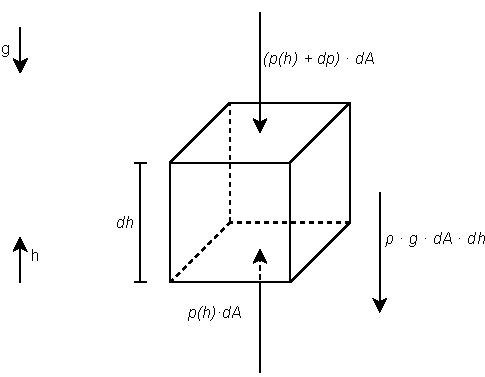
\includegraphics[width=.4\textwidth]{baro_dgl.drawio}
    \caption{Forces around a finitesimally small element}
    \label{fig:baro_FE}
\end{figure}


Please note that the original gravity term of course is $\rho \cdot dV \cdot g$ but we can transform it to $\rho \cdot dA \cdot dh \cdot g$ using the correlation $dV = dA * dh$ with $dA$ being the area of the elements top and bottom side.

From equation \ref{eq:baro_equilibrium}
\begin{equation}
    \sum{F_h} = 0 = p(h) \cdot dA - ( p(h) + dp )\cdot dA -  \rho \cdot g \cdot  dh \cdot dA
    \label{eq:baro_equilibrium}
\end{equation}

follows \ref{eq:baro_equilibrium_simple}.

\begin{equation}
    dp=-\rho \cdot g\cdot dh
    \label{eq:baro_equilibrium_simple}
\end{equation}

$\rho$ can be taken out of eq. \ref{eq:baro_equilibrium_simple} using the perfect gas formula $p=\rho R T$ and equation \ref{eq:baro_equilibrium_perfect} emerges.

\begin{equation}
    \frac{dp}{p} = \frac{-g}{R \cdot T} \cdot dh
    \label{eq:baro_equilibrium_perfect}
\end{equation}


At this point we need to introduce the Temperature model of the ISA. It assumes linear temperature gradients for each layer of the atmosphere, meaning that each atmospheric layer can be modeled using a single coefficient that models the gradient. In the following, this gradient will be used as $a=dT/dh$. This allows modeling the temperature for each atmospheric layer with equation \ref{eq:isa_temperature}.

\begin{equation}
    T(h)= a  \cdot h + T_0
    \label{eq:isa_temperature}
\end{equation}

\begin{table}[h]
    \centering
    \begin{tabular}{@{}cccc@{}}
        \toprule
        Atmospheric  & Geopotential      & Temperature T     & Temperature           \\
        Layer        & Altitude {[}km{]} & at bottom {[}K{]} & gradient a {[}K/km{]} \\ \midrule
        Troposphere  & -2-0              & 301.15            & -6.5                  \\
        Troposphere  & 0-11              & 288.15            & -6.5                  \\
        Tropopause   & 11-20             & 216.65            & 0                     \\
        Stratosphere & 20-32             & 216.65            & 1                     \\
        Stratosphere & 32-47             & 228.65            & 2.8                   \\
        Stratopause  & 47-51             & 270.65            & 0                     \\
        Mesosphere   & 51-71             & 270.65            & -2.8                  \\
        Mesosphere   & 71-80             & 214.65            & -2                    \\ \bottomrule
    \end{tabular}
    \caption{International Standard Atmosphere cite ISO75. Atmospheric Layers model the average physical correlations and do not represent real atmospheric values which vary greatly based on latitude and local factors.}
    \label{tab:isa_temp}
\end{table}


Using the different coefficients from table \ref{tab:isa_temp} we now can model the Temperature based on a standard temperature of 15° Celsius or 288.15Kelvin at Mean Sea Level (MSL), meaning that $h=0$. The temperature gradients drastically simplify real circumstances but work as an empirical estimate that is good enough to guarantee a common understanding of barometric altitudes. This is especially important for aeronautic applications since altitudes for directing flights are generally given in barometric altitudes.

Now, substituting the ISA-equation \ref{eq:isa_temperature} into \ref{eq:baro_equilibrium_perfect} delivers \ref{eq:baro_pde_full}.

\begin{equation}
    \frac{dp}{p}=\frac{-g}{R*(a*h+T_0)}*dh
    \label{eq:baro_pde_full}
\end{equation}

To get this differential equation into a regular formula we need to integrate which resolves into equation \ref{eq:baro_integrated}.

\begin{equation}
    \ln(\frac{p}{p_0}) = - \frac{g}{a \cdot R} \cdot ln(\frac{a*h+T_0}{a*h_0+T_0})
    \label{eq:baro_integrated}
\end{equation}

The borders chosen for integration are the lower border of the atmospheric layer referenced with the index 0 and the other layer being the running variable.

Substitution for the single factors follow in equations\ref{eq:baro_substitutions}.

\begin{equation}
    \ln(a) = b * \ln(c)
    \label{eq:baro_substitutions}
\end{equation}
\begin{conditions}
    a & $p/p_0$                                                                                                                 \\
    b & $\frac{-g}{a \cdot R} $                                                                                                 \\
    c & $\frac{a \cdot +T_0}{a \cdot h_0+T_0} = 1+ \frac{a \cdot (h-h_0)}{a \cdot h_0+T_0} = 1+ \frac{a \cdot (h-h_0)}{T(h_0)}$
\end{conditions}


Subequation c is then simplified by pulling $T_0$ into the denominator and substituting the ISA-equation \ref{eq:isa_temperature}.

After substituting, the term \ref{eq:baro_sub_first} emerges.
\begin{equation}
    \ln(a) = b * \ln(c) = \ln(c^b)
    \label{eq:baro_sub_first}
\end{equation}

Brief transformation then resolves into \ref{eq:baro_sub_last}.
\begin{equation}
    \rightarrow a = c^b
    \label{eq:baro_sub_last}
\end{equation}


Resubstituting then gives equation \ref{eq:baro_Tvar}, the barometric altitude equation.

\begin{equation}
    \frac{p}{p_0}=\left(1+\frac{a \cdot\left(h-h_0\right)}{T\left(h_0\right)}\right)^{\frac{-g}{a \cdot R}}
    \label{eq:baro_Tvar}
\end{equation}

\begin{conditions}
    p      & pressure at current altitude [Pa]                                \\
    p_{0}  & reference pressure [Pa]                                          \\
    h      & current altitude   [m]                                              \\
    h_{0}  & reference altitude [m]                                           \\
    T(h_0) & temperature at reference altitude[K]                             \\
    a      & ISA Temperature Coefficient depending on altitude $(-6.5e-3)[K/m]$ \\
    g      & gravity constant $(9.80665) [m/s^2]$                               \\
    R      & Ideal Gas Constant  $(287.05287)[m^2/( K\cdot s^2)]$
\end{conditions}

Transforming this formula for altitude resolves into equation \ref{eq:h_baro_Tvar}

%\[1 + \frac{a}{T(h_0)}\cdot (h-h_0) = \left(\frac{p}{p_0}\right)^{\frac{1}{\frac{-g}{a \cdot R}}}\]
\begin{equation}
    \rightarrow h = \left(\frac{p}{p_0}^{\frac{-a*R}{g}}-1\right)\frac{T(h_0)}{a}+h_0
    \label{eq:h_baro_Tvar}
\end{equation}

\paragraph{Barometric equation for constant layer temperature}

This formula however is not valid for constant layer temperature and $a=0$. So the barometric equation \ref{eq:baro_pde_full} needs to adapted to $a=0$ \textbf{before} integration. From equation \ref{eq:baro_pde_full} henceforth follows equation \ref{eq:baro_Tconst_pde}.
\begin{equation}
    \frac{dp}{p} = \frac{-g}{RT_0} \cdot dh
    \label{eq:baro_Tconst_pde}
\end{equation}

Integrating then yields \ref{eq:baro_Tconst_integrated}:

\begin{equation}
    \ln\left(\frac{p}{p_0}\right) = \frac{-g}{RT_0} \cdot h
    \label{eq:baro_Tconst_integrated}
\end{equation}

And resolving for pressure into equation \ref{eq:baro_Tconst} follows into the barometric equation for a constant temperature coefficient.

\begin{equation}
    \frac{p}{p_0}= exp\left(\frac{-g}{RT(h_0)}\cdot(h-h_o)\right)
    \label{eq:baro_Tconst}
\end{equation}


The following equation \ref{eq:h_baro_Tconst} then resolves for the altitude based on pressure ratio within a layer with constant temperature.


%$$ln(\frac{p}{p_0}) =\frac{-g}{RT(h_0)}\cdot(h-h_o) $$
\begin{equation}
    h = ln(\frac{p}{p_0})\cdot \frac{RT(h_0)}{-g}+h_0
    \label{eq:h_baro_Tconst}
\end{equation}

\paragraph{Process to determine altitude}

The process to then actually calculate a barometric altitude is displayed in figure \ref{flow:ISA}. The input is p and $p_0$ with p being the measured pressure via the aircrafts static ports and $p_0$ being the reference pressure that is manually set by the pilot with the standard pressure being $p_{std} = 1013.25hPA$ which varies according to the weather.


\begin{figure}[h]
    \centering
    \begin{tikzpicture}[
        node distance=3cm,
        terminal/.style={draw, rounded rectangle,rounded corners=10pt, text centered, minimum height=4em, minimum width=6em},
        io/.style={draw, trapezium, trapezium left angle=70, trapezium right angle=110, minimum height=2em, minimum width=4em},
        process/.style={draw, rectangle, text centered, minimum height=2em, minimum width=5em},
        decision/.style={draw, diamond, aspect=2, text centered, minimum height=2em, minimum width=3em}
    ]
% Nodes
        \node (start) [draw, terminal] {Start};
        \node (input) [draw, io, above of=start] {$p, p_{0}$};
        \node (data) [draw, io, below of=start] {isa};
        \node (getlayer) [draw, process, right of=start, align=center] {[1]\\ get layer from \\table \ref{tab:isa_temp}};
        \node (decide) [draw, decision, right of=getlayer, align=center] {[2] is a=0};
        \node (a) [draw, process, below right of=decide, align=center] {[3.2]   $a=0$\\Get p with eq. \ref{eq:h_baro_Tconst}};
        \node (notA) [draw, process, above right of=decide, align=center] {[3.1]  $a \neq 0$\\Get p with eq. \ref{eq:h_baro_Tvar}};
        \node (output) [draw, io, below right of=notA, align=center] {[4]\\ altitude output};
        \node (stop) [draw, terminal, right of=output] {Stop};

% Arrows
        \draw [->] (start) -- (getlayer);
        \draw [->] (input) -| (getlayer);
        \draw [->] (data) -| (getlayer);
        \draw [->] (getlayer) -- (decide);
        \draw [->] (decide) |- node[anchor=east]{Yes} (a);
        \draw [->] (decide) |- node[anchor=east]{No} (notA);
        \draw [->] (a) -| (output);
        \draw [->] (notA) -| (output);
        \draw [->] (output) -- (stop);
    \end{tikzpicture}

    \caption{Process for determining barometric altitude from pressure and reference pressure only.}
    \label{flow:ISA}
\end{figure}



The current atmospheric layer gets found by matching the MSL-pressure ratio  $\frac{p}{p_0}$ to precalculated boundary values of layers based on table \ref{tab:isa_temp}.
After determining the layer and the value for temperature coefficient $a$, the altitude can quickly be determined by inserting layer properties as well as the pressure ratio into their according altitude equation (step 3.1 and 3.2 in flowchart \ref{flow:ISA}). In the final step 4 the altitude is returned.

Notes: The ISA Norm defines barometric equations for both geometric as well as geopotential conditions. Both start at MSL but geopotential altitude assumes equal acceleration $g$ for every altitude. Since its value as an industry-standard, the gepotential altitude is considered in this work. For completeness the correlation between geopotential and geometric altitude is given in equation \ref{eq:geopotential_alt}. This formula is based on a derivation of gravity potentials and a full derivation can be found in \textcite{iso_standard_1975}.


\begin{equation}
    h_{geometric} = \frac{r_{earth} \cdot h_{geopotential}}{r_{earth} - h_{geopotential}}
    \label{eq:geopotential_alt}
\end{equation}
\newpage



\section{Structuring large datasets}

\subsection{Data Format, FAIR}

Originating from a dutch alliance of biotechnology institutes in 2015, the FAIR Guiding principles emerged in 2016 as a general best practice guide for research data, referencing best practices

FAIR principles have been published in 2016 by the source here. They set the foundation for a standardized and open data culture. Within these principles values like open access for data, findable and well tagged datasets, interoperable data by using standardized formats and or semantics (define semantics as well) which guarantee a reusability of data to generate a sustainable process for data usage. Effectively meaning that similar experiments do not have to be performed multiple times when well tagged and formatted data is freely available.


json file format (FAIR-principles, INST-DLR, SOIL)

Explain which means are taken to guarantee an architecture throughout the work that ensures an implementation of the FAIR principles and the V-model.
Architecture of the JSON-Tree structure and which data is inserted where.


-modern data management principles (storage not as important as readability)

Comparison with existing data structures. Implementation into existing architecture

--> Chosen Data Model, Semantics



\subsection{SOIL}

\subsection{Skystash}
\label{chap:skystash}

Flight test data needs to be perceived within the context of its circumstances to extract all its information.

dlrk paper hier zitieren.

this work(flight data, sensor positions, isa table)

\begin{figure}[h]
    \centering
    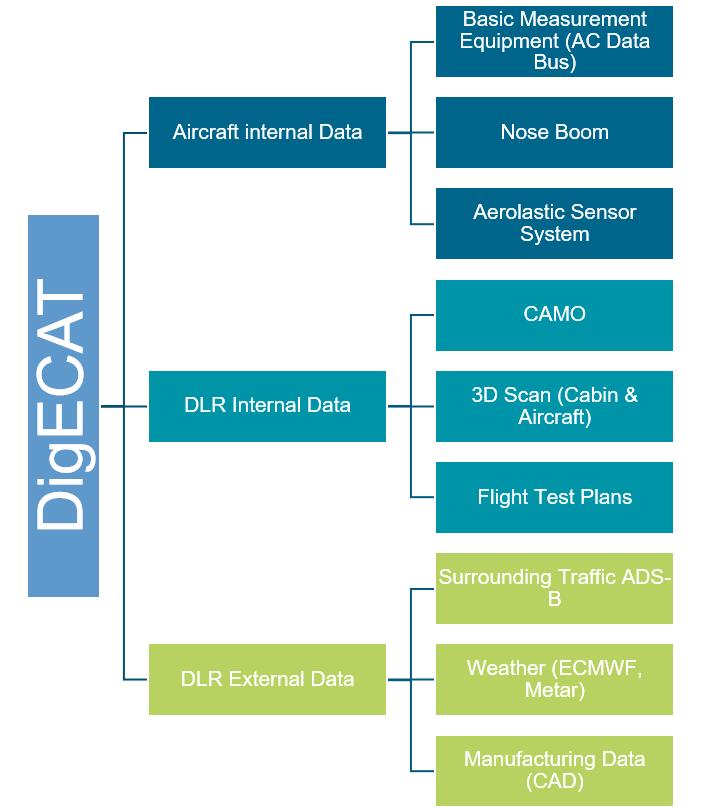
\includegraphics[width=\textwidth]{03_figures/DIGECAT}
    \caption{Generation of flight test data \cite{arts_digital_nodate} }
    \label{fig:digecat_data_sources}
\end{figure}
!!!!!!!!do a part page design here.


\begin{figure}[h]
    \centering
    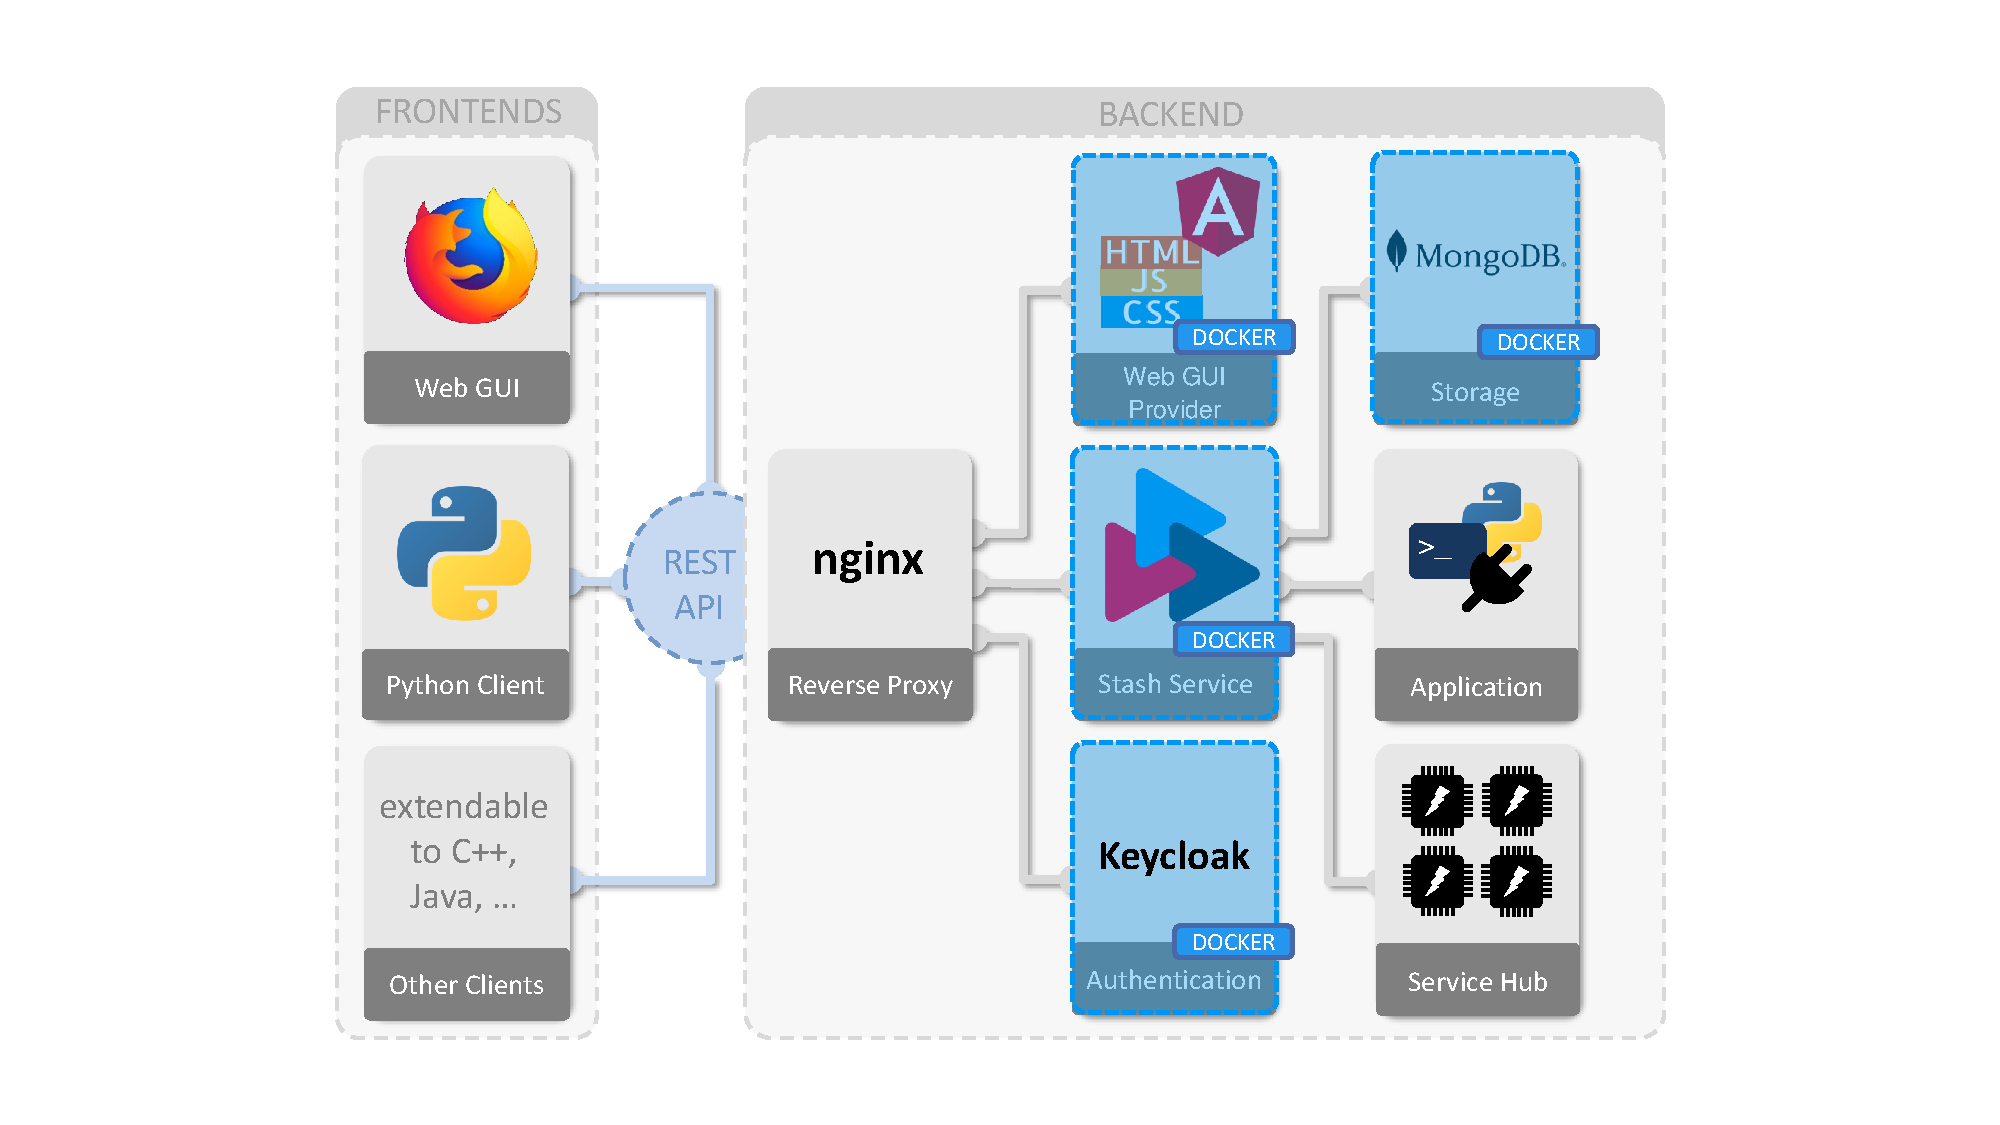
\includegraphics[width=\textwidth]{03_figures/stash_architecture}
    \caption{The Skystash architecture \cite{arts_digital_nodate}}
    \label{fig:stash_architecture}
\end{figure}

the skystash is a platform to distribute, analyze and visualize large flight data sets. It is currently in development within the DLR's digital twin project and aims to be a service platform for uploading and sharing the DLR's flight test data. Various requirements are posed from different stakeholders such as the topic of sampling rate. Flight guidance projects may be content with sampling rates as low as 1 Hz. Other stakeholders such as aeroelastic experts may require sampling rates as high as possible and may reach up to 2000Hz within the ISTAR. For this purpose a dynamic data export is sensible in which users can directly choose sampling rates as well as single parameters from a flight contrary to downloading and working with a whole flight data set averaging up to 2GB of data.

This work builds upon the python api and tries to implement and test an algorithm that checks the data for the istar aircraft


%\section{downloadfunctionalities}
file sizes too large --> Reduction for on demand parameters and resampling utility
Handling of large data sets

\subsection{optimal data structure}
data
metadata
needs to be efficient

\subsection{A word towards unit management}

Units, especially within aerospace contexts, are far from standardized. Most scientific users prefer SI-units. However, the convention for Pilots and Flight Test Engineers remains imperial within units such as feet, Nautical Miles, knots and so on. Table \ref{tab:unit_conversions} gives an overview over the conversions that are used within this work. Naturally SI-units are chosen for calculations since calculations are more efficient as well as less prone to errors in SI-systems.

\begin{table}
    placeholder
    \label{tab:unit_conversions}
\end{table}




\section{conclusion theory and basics}

BAsed upon these fundamentals, the effort is undertaken to implement the Sensor Health  Monitoring
